\section{Durchführung}
\label{sec:Durchführung}

\begin{figure}[H]
  \centering
  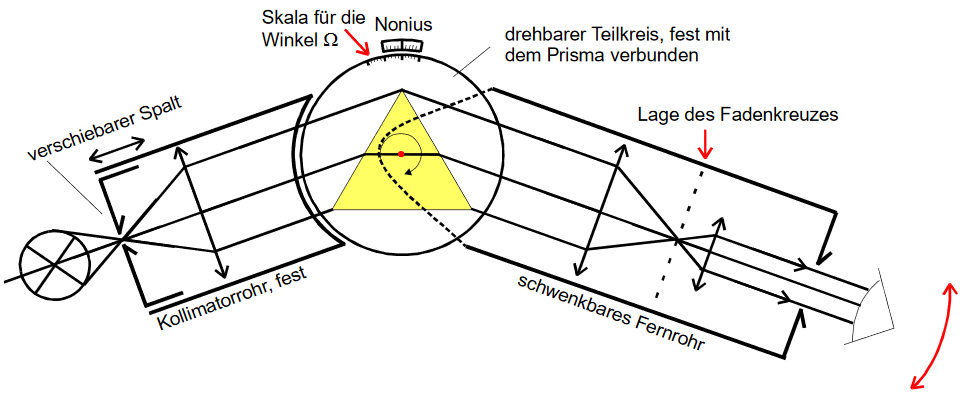
\includegraphics[height=5cm]{Aufbau.PNG}
  \caption{Schematische Darstellung eines Prismen-Spektralapparats \cite{sample}.}
  \label{fig:aufbau}
\end{figure}

Bei diesem Versuch wird eine Apparatur verwendet, dessen schematischer Aufbau in Abbildung \ref{fig:aufbau}
dargestellt ist. Aus einer Hg-Cd-Sprektrallampe fällt Licht auf einen Spalt, welcher wiederum in der Brennebene
einer Kollimatorlinse leigt. Dadurch wird hinter der Linse ein paralleler Strahlengang des Lichts hergestellt.
Anschließend fällt dieses auf ein Prisma und wird dort zwei mal gebrochen, bevor es ein bewegliches Fernrohr
durchläuft, an dessen Ende das es dann mit dem Auge beobachtet werden kann. Dabei lässt sich dann
an der Drehscheibe des Fernrohrs der Winkel ablesen auf dem es gerade steht.

\begin{figure}[H]
  \centering
  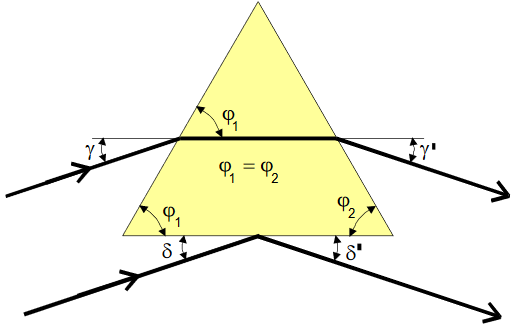
\includegraphics[height=5cm]{Brechung.PNG}
  \caption{Symmetrischer Strahlengang am Prisma \cite{sample}.}
  \label{fig:brechung}
\end{figure}

Zu Beginn des Versuchs wird die Winkeländerung bestimmt, die das Licht der einzelnen Wellenlängen beim durchlaufen des Prismas
erfährt. Dazu wird für jede einzelne sichtbare Spektrallinie ein möglichst symmetrischer Strahlengang erzeugt (Abbildung \ref{fig:brechnung}).
Das im Prisma gebrochene und das an der Prismaoberfläche reflektierte Licht sollen also möglichst parallel in des Fernrohr einlaufen.
Sodann wird für jede Spektrallinie der Winkel abgelesen, unter dem das Fernrohr in diesen besagten Einstellungen gerade steht.
Anschließend wird die gleiche Messung noch einmal bei spiegelsymmetrischer Stellung des Prismas durchgeführt (zu erkennen in Abbildung \ref{fig:eta}).
Aus diesen beiden gemessenen Winkeln kann dann schließlich die tatsächliche Winkeländerung bestimmt werden.

\begin{figure}[H]
  \centering
  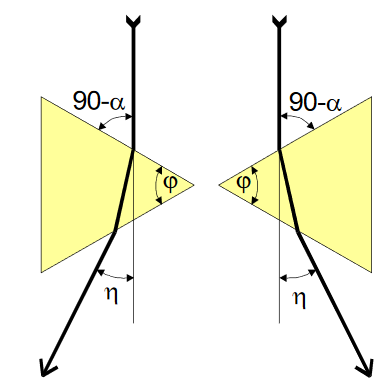
\includegraphics[height=5cm]{eta.PNG}
  \caption{Prinzip der Messung der beiden Ablenkungswinkel \cite{sample}.}
  \label{fig:eta}
\end{figure}

Als letztes soll dann noch der Innenwinkel des Prismas festgestellt werden. Dazu positioniert man das Prisma mit einer seiner Spitzen in
Richtung des eintreffenden Lichts (Abbildung \ref{fig:phi}). Anschließend misst man analog zur ersten Messung die Winkel, unter denen auf beiden Seiten jeweils
die Reflektion des Lichtes zu finden ist. Man wiederholt die Messung anschließend für weitere sechs (leicht geänderte) Ausrichtungen
des Prismas. Aus diesen Winkeln lässt sich dann schließlich der Innenwinkel bestimmen.

\begin{figure}[H]
  \centering
  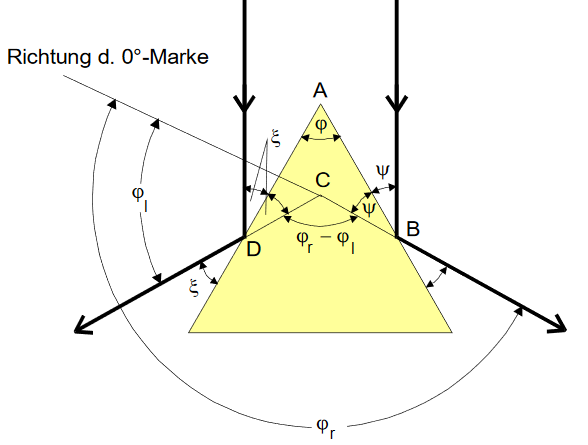
\includegraphics[height=5cm]{phi.PNG}
  \caption{Lichtreflektion bei der Bestimmung des Innenwinkels des Prismas \cite{sample}.}
  \label{fig:phi}
\end{figure}
